\documentclass{bioinfo}
% * <michalburdukiewicz@gmail.com> 2016-03-25T10:03:29.805Z:
%
% ^.
\copyrightyear{2015} \pubyear{2015}
\usepackage{graphicx}
\usepackage{booktabs}
\usepackage{colortbl, xcolor}
\access{Advance Access Publication Date: Day Month Year}
\appnotes{Manuscript Category}

\newcommand*{\bigcdot}{\raisebox{-0.25ex}{\scalebox{1.5}{$\cdot$}}}

\begin{document}
\firstpage{1}

\subtitle{Subject Section}

\title[Prediction of amyloidogenicity based on the n-gram analysis]{Prediction of amyloidogenicity based on the n-gram analysis}
\author[Sample \textit{et~al}.]{Micha\l{} Burdukiewicz$^{\text{\sfb 1,*}}$, Piotr Sobczyk\,$^{\text{\sfb 2}}$, Pawe\l{} Mackiewicz$^{\text{\sfb 1}}$ and Ma\l{}gorzata Kotulska\,$^{\text{\sfb 3,}*}$}
\address{$^{\text{\sf 1}}$University of Wroc\l{}aw, Department of Genomics,
$^{\text{\sf 2}}$Wroc\l{}aw University of Technology, Department of Mathematics and 
$^{\text{\sf 3}}$Wroc\l{}aw University of Technology, Department of Biomedical Engineering, Faculty of Fundamental Problems of Technology
}

\corresp{$^\ast$To whom correspondence should be addressed.}

\history{Received on XXXXX; revised on XXXXX; accepted on XXXXX}

\editor{Associate Editor: XXXXXXX}

\abstract{\textbf{Motivation:} Tekst
Text Text Text Text Text Text Text Text Text Text Text Text Text Text Text Text Text Text Text
Text Text Text Text Text Text
Text Text Text Text Text.\\
\textbf{Results:} Text  Text Text Text Text Text Text Text Text Text  Text Text Text Text Text vvv
% * <michalburdukiewicz@gmail.com> 2016-02-23T09:35:35.738Z:
%
% ^.
Text Text Text Text Text Text Text Text Text Text Text Text Text  Text Text Text Text Text Text\\
\textbf{Availability:} Text  Text Text Text Text Text Text Text Text Text  Text Text Text Text
Text Text Text Text Text Text Text Text Text Text Text Text Text Text  Text\\
\textbf{Contact:} \href{name@bio.com}{name@bio.com}\\
\textbf{Supplementary information:} Supplementary data are available at \textit{Bioinformatics}
online.}

\maketitle

\section{Introduction}


%\enlargethispage{12pt}
Amyloid aggregates have been observed in tissues of people suffering from 
Alzheimer's disease, Parkinson's disease, amyotrophic lateral sclerosis and 
Huntington's disease, as well as many other conditions. They also include 
diseases other than neurological, for example diabetes type 2 or certain types 
of a cataract. Cells in tissues with amyloid fibrils exhibit very high 
mortality. However, the mechanisms of the cytotoxicity have not been discovered. 
Unfortunately dissolution of the aggregates is very difficult. Amyloids are 
resistant to activity of proteolytic enzymes and chemical compounds due to the 
specific and highly ordered structure of their steric zipper.

  The aggregation occurs when a cell environment fosters the partial unfolding 
of protein chains or their fragmentation, in a way that the parts prone to 
joining with other protein fragments are exposed. For the majority of proteins, 
considerable conformational rearrangement must have occurred to initiate the 
aggregation process. Such changes cannot take place in the typical tightly 
packed native protein conformation, due to the constraints of the tertiary 
structure. Thus, formation of a non-native partially unfolded conformation is 
required, presumably enabling specific intermolecular interactions, including 
electrostatic attraction, hydrogen bonding and hydrophobic contacts. This 
partial unfolding can be influenced by various factors, such as protein high 
concentration, high temperature, low pH, binding metals, or exposition to UV 
light.

  Initially, the resulting molecules form clusters consisting of a few 
elements, which are called oligomers. Next, they grow into larger aggregates. 
Aggregation of proteins or their fragments may lead to amorphous (unstructured) 
clusters or amyloid (highly ordered) unbranched fibrils. Independently of the 
protein sequence and its original structure, aggregates always display a common 
cross-$\beta$ structure. The distinctive structure of the steric zipper enables 
the selective detection of amyloids from amorphous aggregates using either a 
variety of microscopic techniques or fluorescence of probes with which they form 
compounds.

  Currently, it is believed that short peptide sequences of amyloidogenic 
properties (called hot-spots) can be responsible for aggregation of amyloid 
proteins.  Previous studies have suggested that amyloidogenic fragments may have 
regular characteristics, not only with regard to averaged physicochemical 
properties of their amino acids, but also the order of amino acids in the 
sequence. There have been attempts to predict the sequence of such peptides by 
computational modelling. Physics and chemistry based models have been used, 
including FoldAmyloid~\citep{garbuzynskiy_foldamyloid:_2010}. This method is 
based on the density of the protein contact sites. Other methods perform 
threading a peptide on an amyloid fiber backbone, followed by determination of 
its energy and stability~\citep{goldschmidt_identifying_2010, 
bryan_stitcher:_2012, odonnell_method_2011}. Statistical approaches include 
production of frequency profiles, such as the WALTZ method 
\citep{beerten_waltz-db:_2015} and machine learning methods, which have been 
used by our team \citep{stanislawski_machine_2013, gasior_fish_2014}. Some other 
approaches, mostly biophysical-based, enable classification of hot spots for 
non-amyloid aggregation. Recently, AGGRESCAN3D has been proposed to estimate 
more accurately aggregation propensity by performing 3D structure based 
analysis~\citep{zambrano_aggrescan3d_2015}. 
% * <kotulska@gmail.com> 2016-03-29T15:34:04.588Z:
%
% > Many diseases, especially neurodegenerative, result from protein fragments forming aggregates. This occurs when a cell environment fosters the partial unfolding of protein chains or their fragmentation, in a way that the parts prone to joining with other protein fragments are exposed. For the majority of proteins, considerable conformational rearrangement must have occurred to initiate the aggregation process. Such changes cannot take place in the typical tightly packed native protein conformation, due to the constraints of the tertiary structure. Thus, formation of a non-native partially unfolded conformation is required, presumably enabling specific intermolecular interactions, including electrostatic attraction, hydrogen bonding and hydrophobic contacts. This partial unfolding can be influenced by various factors, such as protein high concentration, high temperature, low pH, binding metals, or exposition to UV light.
% > Initially, the resulting molecules form clusters consisting of a few elements, which are called oligomers. Next, they grow into larger aggregates. Aggregation of proteins or their fragments may lead to amorphous (unstructured) clusters or amyloid (highly ordered) unbranched fibrils. Independently of the protein sequence and its original structure, aggregates always display a common cross-$\beta$ structure. The distinctive structure of the steric zipper enables the selective detection of amyloids from amorphous aggregates using either a variety of microscopic techniques or fluorescence of probes with which they form compounds.
% > Amyloid fibrils have been observed in the brains of people suffering from Alzheimer's disease. They are also associated with Parkinson's disease, amyotrophic lateral sclerosis and Huntington's disease, as well as many other conditions, even 
% > non-neurodegenerative diseases such as type 2 diabetes and some types of cataract. Cells in tissues containing these fibrils exhibit very high mortality. However, the reasons for this cytotoxicity have not been resolved. In recent years the occurrence rate of diseases characterized by accumulation of protein deposits has increased significantly. These disorders are sometimes called diseases of civilization since they are more prevalent in developed countries where life expectancy is higher. Unfortunately, their mechanisms are still poorly understood. Although studies indicate that these diseases to some extent have a genetic basis, the influence of lifestyle cannot be excluded. Unfortunately dissolution of peptide aggregates is very difficult, especially for amyloids which are resistant to activity of proteolytic enzymes and chemical compounds due to the specific and highly ordered structure of their steric zipper.
%
% Ten tekst jest na razie przykładowy, oparty na moim tekscie juz użytym. 
%
% ^ <kotulska@gmail.com> 2016-04-01T13:21:05.364Z.
% * <kotulska@gmail.com> 2016-03-29T14:52:35.515Z:
%
% Tu konicznie trzeba napisać wprowadzenie do metody n-gramów i tego co wcześniej z Piotrem już zrobiliście i opublikowaliście
%
% ^.

  In this study we present an n-gram model of amyloidogenic sequences. In 
bioinformatics n-grams (k-mers) are continuous or discontinuous sequences of $n$ 
elements. Employed as a feature extraction method, n-grams are widely used in 
analysis of biological sequences. The choice of n-grams was driven by their 
highly interpretable nature, because we were interested in the identification of 
motifs most relevant to amyloidogenic properties. We selected these n-grams 
using the novel feature selection algorithm called Quick Permutation Test 
(QuiPT).

  Several studies highlighted that three-dimensional protein structure depends 
not on the exact sequence of amino acids, but on their general physicochemical 
properties. Hence, a reduced amino acid alphabet, where a single element 
represents several amino acids, still retains the information about protein 
folding~\citep{murphy_simplified_2000}. Since amyloid aggregates, especially 
their hot-spots regions, have very specific spatial organization, we 
investigated if it also can be described using shorter alphabet. Instead of 
relying on general similarities of amino acids, we created our own reduced amino 
acid alphabets based on the combinations of properties that might be associated 
with amyloidogenicity. Due to that we discovered which physicochemical 
properties discriminate the best between amyloids and non-amyloids.

  Our model of amyloidogenicity consisted of n-gram datasets extracted from 
sequences encoded using different reduced amino acid alphabets. The information 
in models was further used to train predictors of amyloids based on random 
forest~\citep{breiman_random_2001}. We trained several iterations of each 
classifier using peptides of different length to identify the optimal number of 
residues consisting the information of the hot-spot presence or absence. 
Through the cross-validation of predictors we determined the best-performing 
classifier, its reduced amino acid alphabet and set of important n-grams.

\begin{methods}
\section{Methods}
\subsection{Data set}

The data used in the study was extracted from AmyLoad data 
base~\citep{wozniak_amyload:_2015}. Aside from eight sequences shorter than five 
residues that were removed from the final data set, we obtained 418 
amyloidogenic sequences and 1039 non-amyloidogenic sequences (1457 peptides in 
total).

  Sequences shorter than 6 amino acids and longer than 25 amino acids were 
removed from the data set. The former were too short to be processed in the 
devised analysis framework and the latter were too diversified and rare, 
hampering the proper analysis.

  The final data set contained 397 amyloidogenic and 1033 non-amyloidogenic 
sequences (1430 peptides in total).

\subsection{Encodings of amino acids}

The amyloidogenicity of a given peptide may not depend on the exact sequence of 
amino acids, but on its more general properties. To verify this hypothesis, we 
created 524 284 reduced amino acid alphabets (encodings) with different lengths 
(from three to six letters) using Ward's 
clusterization~\citep{jr_hierarchical_1963} on the selected physicochemical 
properties from AAIndex database~\citep{kawashima_aaindex:_2008}. We handpicked 
several measures belonging to more general categories important in the  
amyloidogenicity, such as size, hydrophobicity, solvent surface area, frequency 
in $\beta$-sheets and contactivity. As a rule of thumb, we limited it to 
properties introduced after 1980 when, thanks to the technological advancements, 
the measurements were more accurate.

  The majority of encodings had at least one duplicate. In such a case, only a 
single representative was included in the cross-validation. After filtering 
duplicates, we obtained 18 535 unique encodings.
\begin{table*}[bth]
\centering
\begin{tabular}{ll}
  \hline
Category & Property \\ 
  \hline
  Contactivity & Average flexibility indices \citep{bhaskaran_positional_1988} \\ 
  Contactivity & 14 A contact number \citep{nishikawa_radial_1986} \\ 
  Contactivity & Accessible surface area \citep{radzicka_comparing_1988} \\ 
    Contactivity & Buriability \citep{zhou_quantifying_2004} \\ 
  Contactivity & Values of Wc in proteins from class Beta, cutoff 12 A, separation 5 \citep{wozniak_characteristics_2014} \\ 
  Contactivity & Values of Wc in proteins from class Beta, cutoff 12 A, separation 15 \citep{wozniak_characteristics_2014} \\ 
  $\beta$-frequency & Average relative probability of inner beta-sheet \citep{kanehisa_local_1980} \\ 
  $\beta$-frequency & Relative frequency in $\beta$-sheet 
\citep{prabhakaran_distribution_1990} \\ 
  $\beta$-frequency & Thermodynamic $\beta$-sheet propensity 
\citep{kim_thermodynamic_1993} \\ 
  Hydrophobicity & Hydrophobicity index \citep{argos_structural_1982} \\ 
  Hydrophobicity & Optimal matching hydrophobicity \citep{sweet_correlation_1983} \\ 
  Hydrophobicity & Hydrophobicity-related index \citep{kidera_statistical_1985} \\ 
  Hydrophobicity & Scaled side chain hydrophobicity values \citep{black_development_1991} \\ 
  Polarity & Polarizability parameter \citep{charton_structural_1982} \\ 
  Polarity & Mean polarity \citep{radzicka_comparing_1988} \\ 
  Size & Average volumes of residues \citep{pontius_deviations_1996} \\ 
  Stability & Side-chain contribution to protein stability (kJ/mol) \citep{takano_new_2001} \\ 
   \hline
\end{tabular}
\caption{Physicochemical properties used in the creation of reduced amino acid 
alphabets.} 
\label{tab:properties}
\end{table*}

  Since correlated or, contrarily, uncorrelated measures create very similar 
encodings, we further reduced the number of properties to 17 by selecting 
measures with the absolute value of Pearson's correlation coefficient larger 
than 0.95 for normalized values (Tab.~\ref{tab:properties}).

\subsection{Training of learners}

\begin{figure}[!tpb]
\centerline{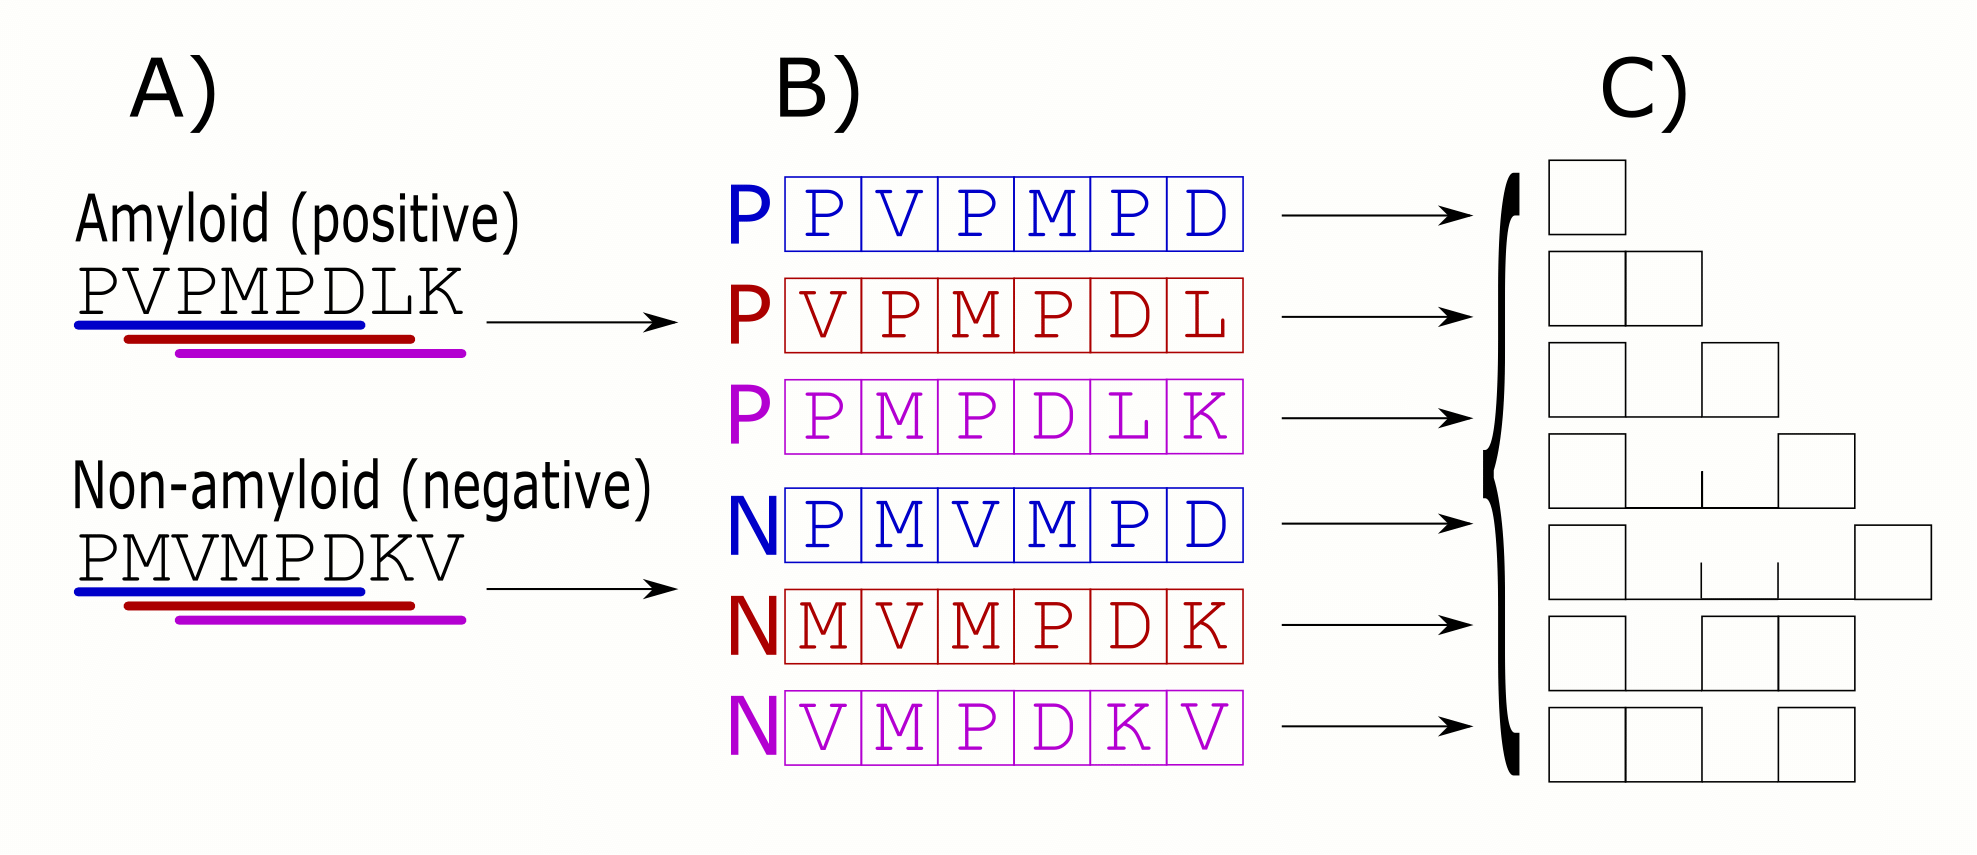
\includegraphics[width=\columnwidth]{figures/ngram_scheme.png}}
  \caption{The scheme of n-gram extraction. A) Input data - peptides with a 
known amyloidogenicity status. B) Each peptide sequence was divided into 
overlapping hexamers. The amyloidogenicity status of a source sequence was used 
as the amyloidogenicity status of a derived hexamer. C) From each hexamer we 
extracted continuous 1-, 2- and 3-grams. We selected also gapped 2-grams with 
the length of gap equal from 1 to 3 residues and gapped 3-grams with a single 
gap between the first and the second or the second and the third element of the 
n-gram.}
\label{fig:ngram_scheme}
\end{figure}

During the training phase, we extracted overlapping hexamers from each sequence. 
Each hexamer was tagged with the same etiquette (amyloid/nonamyloid) as the 
source peptide. For example, the amyloidogenic sequence of length 6 residues 
yields only one 
% * <kotulska@gmail.com> 2016-03-29T12:38:15.711Z:
%
% > original peptide
%
% czemu? co to oznacza?
%
% ^ <michalburdukiewicz@gmail.com> 2016-03-31T16:51:58.668Z:
%
% każdy heksamer dostał taką samą etykietę jak peptyd z którego pochodzi. Np. z peptydu amyloidogennego o długości 8 wyodrębniono 3 heksamery i każdemu z nich przypisano etykietę "amyloidogenny"
%
% ^.
hexamer tagged as "amyloid". The non-amyloidogenic sequence of 8 residues yields 
3 hexamers, all marked as "non-amyloids". (Fig.~\ref{fig:ngram_scheme} A and B). 
Assuming that in longer amyloids only a short part of the sequence is 
responsible for amyloidogenicity, our method might result in many false 
positives in the training data set. To evade this problem, we restricted the 
maximum length of peptides in training data set to fifteen amino acids to easy 
the extraction of probable hot-spots.

  From each hexamer we extracted n-grams of the following length: 1, 2 and 3. In 
the case of 2- and 3-grams, we separately counted both gapped and continuous 
n-grams. For 2-grams we counted n-grams with gaps of lengths from 1 to 3 and for 
3-grams with a single gap between the first and the second or the second and the 
third element (see Fig.~\ref{fig:ngram_scheme}).

  To study the length of amyloidogenic signal, we trained three 
classifiers for each encoding on the sequences of different lengths. We 
considered separately six-residue sequences, shorter or equal to ten residues 
and shorter or equal to fifteen residues.

  All n-grams extracted from the hexamers in the training data set were filtered 
using described below Quick Permutation Test with the information gain (mutual 
information) as the criterion of the importance of a specific n-gram. In the 
next step, we used n-grams with the p-value smaller than 0.05 to build a random 
forest classifier using ranger \textbf{R} package~\citep{wright_ranger:_2015}. 

  Furthermore, we repeated the procedure described above on two typical reduced 
alphabets of amino acids derived from the literature to check if the process of 
% * <kotulska@gmail.com> 2016-03-29T13:34:31.436Z:
%
% > wo typical reduced 
% > alphabets of amino acids derived from the literature
%
% Niezbyt rozumiem. Trzeba byloby dorzucic cytowanie i krótkie wyjasnienie
%
% ^.
amyloidogenicity does require nonstandard groupings of amino acids. We also 
added the full amino acid alphabet to assess the advantages of the amino acid 
encoding.

\subsection{Quick Permutation Test (QuiPT)}

The permutation tests, commonly used for filtering important n-grams, are 
computationally expensive, and, as a result, they often become one of the most
limiting factors for these kinds of analysis. 
The Quick Permutation Test effectively filters 
n-gram features without performing a huge number of permutations. Let us 
consider the contingency table for target $y$ and feature $x$. For example 
entry $n_{10}$ is the number of cases when target is $1$ and feature is $0$.

\begin{center}
\begin{tabular}{ | c || c | c | c | }
  \hline			
  target / feature & 1 & 0 & total\\ \hline
 1 & $n_{1,1}$ & $n_{1,0}$ & $n_{1,\bigcdot}$ \\
 0 & $n_{0,1}$ & $n_{0,0}$ & $n_{0,\bigcdot}$ \\ \hline
 total & $n_{\bigcdot,1}$ & $n_{\bigcdot,0}$ & $n$ \\
  \hline  
\end{tabular} 
\end{center}

  Under the hypothesis that $x$ an $y$ are independent, the probability of 
observing such a contingency table is given by the multinomial distribution. The 
idea of permutation test is to reshuffle feature and target labels, while 
keeping the total number of positives in both of them fixed. When we impose this 
constraint on the multinomial distribution, then the probability of occurrence 
for a given contingency table depends only on one entry, say $n_{1,1}$, and is 
fairly easy to compute. After computing Information Gain (IG) for each possible 
value of $n_{1,1} \in [0,min(n_{\bigcdot, 1}, n_{1, \bigcdot})]$, we get the 
distribution of Information Gain under hypothesis that target and feature are 
independent. We reject null hypothesis, when IG for a feature we test is above a 
required quantile from IG distribution.

  Having the analytical formula for the distribution, allows us to perform 
permutation test much quicker. Furthermore, we get exact quantiles even for 
extreme tails of the distribution, which is not guaranteed by random 
permutations. In fact, imagine performing the test with $\alpha=10^{-8}$, which 
is not an uncommon value, e.g. when one adjusts for multiple testing. Even for a 
huge number of permutations like $m=10^8$, the standard deviation of quantile 
estimate in permutation test, $\frac{p(1-p)}{m}$, is roughly equal to $\alpha$ 
itself.

  In the context of k-mer data we can speed up our algorithm even further. Note 
that since target $y$ is common for testing all k-mer features, test statistics 
depends only on $n_{\cdot, 1}$ -- the number of positive cases in a feature. 
Though we test millions of features, there are just few distributions that we 
need to compute, as usually number of positives in k-mer feature is small. We 
take advantage of this fact and we compute quantiles for just a handful of 
distributions. Therefore complexity of our algorithm is roughly equal $O(n\cdot 
p)$.

  Lastly, let us point out that QuiPT is very similar for Fisher's exact test. 
From the derivation provided in e.g.~\citep{lehmann2008testing}, it becomes 
obvious, that QuiPT is a heuristics for an unsolved problem of a two-tailed 
Fisher's exact test. In this heuristics, extremity of a contingency table, is 
defined by its Information Gain.

\subsection{Cross-validation and selection of the best-performing encoding}

The ability to correctly predict amyloidogenicity was assessed during the 
five-fold cross-validation. Since the data set was very heterogeneous, we 
repeated the cross-validation fifteen times for each classifier to obtain more 
precise estimates of performance measures for each classifier. 

  To evaluate if our classifiers are able to use decision rules extracted from 
sequences of given length to correctly classify longer or shorter sequences, we 
calculate performance measures separately for four ranges of lengths of 
sequences: 6, 7-10, 11-15 and 16-25. The number of sequences from the given 
length range was roughly comparable between folds of cross-validation.
  
  To choose the most adequate reduced amino acid alphabet, we ranked the values 
of Area under Curve - AUC (with rank 1 for the best AUC, rank 2 for the second 
best AUC and so on) for each range of sequence length in the testing data set. 
The encoding with the lowest sum of ranks from all sequence length categories 
was selected as the best one. For this encoding, we choose the range of peptides 
length in the training set providing the best AUC in cross-validation.

\subsection{Encoding distance}
The encoding distance is a measure defining the similarity between two 
encodings. It has zero value for identical encodings and grows with the 
differences between encodings. It was introduced to verify if the reduced 
alphabets very similar to the best-performing encoding will also have good 
prediction performance.

  We define the encoding distance as the minimum number of amino acids that 
have to be moved between subgroups of encoding to make \textit{a} identical to 
\textit{b} (the order of subgroups in the encoding and amino acids in a group 
is unimportant). This measure is further scaled by a factor reflecting how 
much moving amino acids between groups altered mean group properties. 

To compute the scale factor $s$ for the encoding distance between 
encoding \textit{a} with $n$ subgroups and encoding \textit{b} with $m$ 
subgroups we firstly calculate $p_i$ and $p_j$, mean values of physicochemical 
properties of all amino acids separately for each subgroup. The factor between 
$a$ and $b$ is equal to: 

$$
s_{ab} = \sum^n_{i = 1}  \left( \min_{j=1,\dots,m} \left(\sqrt{\sum^l p_{i}^2} 
- \sqrt{\sum^l p_{j}^2} \right) \right)
$$
 
where $l$ is equal to the number of physicochemical properties of concern.

\subsection{Benchmark of AmyloGram}

The best-performing reduced amino acid alphabet chosen during the 
cross-validation was later used to train AmyloGram, n-gram based predictor of 
amyloidogenicity.

  We used \textit{pep424} data set~\citep{walsh_pasta_2014} to compare the 
performance of AmyloGram and other predictors of amyloidogenicity. Since the 
model of AmyloGram does not cover peptides shorter than five amino acids, we 
removed them from the total benchmark data set. It should have not affect the 
comparison as only five sequences were eliminated (around 1\% of the original 
data set). Additionally, we also benchmarked three predictors learned on the 
n-grams extracted from sequences of different length ranges without any amino 
acid encoding.

  All benchmarked classifiers were trained on sequences used during the 
cross-validation. Since some peptides were common for both \textit{pep424} and 
AmyLoad, we removed them from the training data set. After purification, the 
learning data set had 269 positive sequences and 746 negative sequences longer 
than five residues and shorter than fifteen residues. Aside from the 
preparation of the training data, we exactly repeated the procedure of n-gram 
extraction as described above (see Fig.~\ref{fig:ngram_scheme}). 


\end{methods}

\section{Results and discussion}

\subsection{Selection of the best-performing encoding}

\begin{figure*}[!tpb]
\centerline{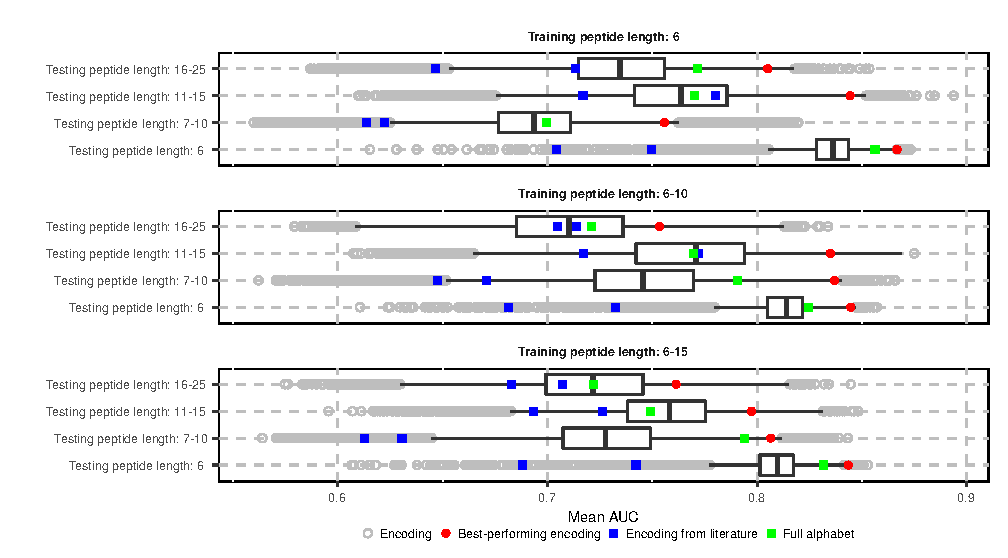
\includegraphics{figures/AUC_boxplot.eps}}
\caption{Distribution of AUC values of different reduced amino acid alphabets 
% * <kotulska@gmail.com> 2016-03-29T14:05:35.815Z:
%
% > \caption{Distribution of AUC values of different reduced amino acid alphabets 
% > for different lengths of sequences in the training and testing data sets.
%
% Jak odczytywać boxplot skoro na wykresie są 4 alfabety? 
%
% ^ <michalburdukiewicz@gmail.com> 2016-03-31T17:22:30.733Z:
%
% Każdy z podwykresów przedstawia wszystkie alfabety. Większość z nich jest niewidoczna, bo jest "ukryta" w wykresie pudełkowym. Kolorami zaznaczyłem alfabety z literatury, najlepszy alfabet i pełny alfabet.
%
% ^.
for different lengths of sequences in the training and testing data sets.
%Red circle: classifier employing best encoding of amino acid. Green square: 
%classifier using full amino acid alphabet. Blue square: classifiers employing 
%encodings from literature.
}\label{fig:AUC_boxplot} 
\end{figure*}


\begin{figure*}[!tpb]
\centerline{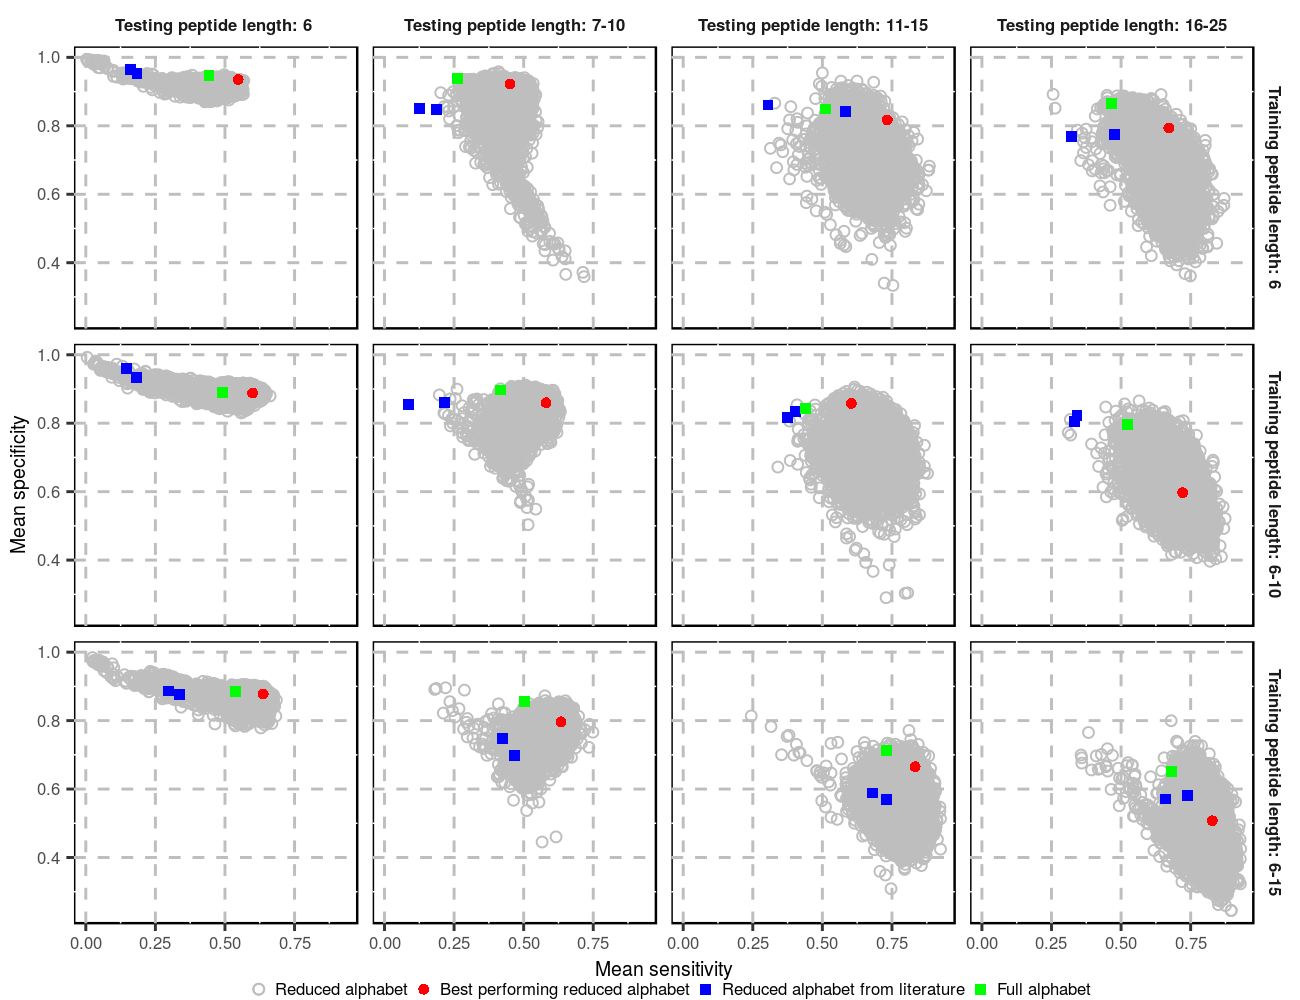
\includegraphics{figures/sesp_plot.png}}
\caption{Sensitivity and specificity of classifiers in cross-validation for 
different lengths of sequences in the training and testing data sets.
%Red 
%circle: classifier employing best encoding of amino acid. Green square: 
%classifier using full amino acid alphabet. Blue square: classifiers employing 
%encodings from literature. 
The classifier based on the best-performing encoding always have 
good specificity and sensitivity.}\label{fig:sesp_plot}
\end{figure*}

The selected encoding performed better than other reduced alphabets considering 
all sequence length ranges in training and testing data set. It had the AUC 
always in the fourth quartile (Fig.~\ref{fig:AUC_boxplot}). For the 
best-performing encoding the most problematic was correct prediction of the 
amyloidogenicity in the longest peptide data set 16-25, not when learned on very 
short sequences, but for longer ones (6-10 and 6-15). Such a behavior was 
typical for most of the analyzed encodings.

  The highest values of AUC the chosen encoding reaches in the relatively the 
simplest cases of predicting amyloidogenicity of the shortest sequences (6 
residues). Of course, the decision rules were the easiest to extract when also 
the learning data set had only sequences of the same lengths, but the results 
were quite comparable even if the training set contained longer sequences. Also 
in this situation, the majority of reduced amino acid alphabets behaved like the 
selected encoding and also had higher AUC than in other scenarios.

  Considering only the AUC value, the most problematic testing data were 
sequences longer than 15 amino acids. Surprisingly, the classifiers trained on 
the shortest sequences available (six residues) were performing the best. That 
might indicate that our n-gram approach extracts the important features the 
better, the shorter are sequences in training data set. For example, in the 
amyloidogenic peptide of length 15, only a very specific region of residues 
might be responsible for the creation of harmful aggregates. In this case, when 
in our framework overlapping n-grams are extracted, only part of them may carry 
the true signal of amyloidogenicity, but all are marked as amyloids. 
Despite this problem, the overall prediction of classifiers learned on the long 
sequences was still adequate, with the median values of AUC higher than 0.7 for 
every testing set. 

  In addition to the high AUC, the best encoding had also very good sensitivity 
and specificity regardless of the length of sequences in training and testing 
set (Fig.~\ref{fig:sesp_plot}). The classifiers trained on the peptides of 
length 6 tend to have the best specificity, while predictors learned on the long 
sequences have the best sensitivity. Albeit the classifiers trained on 
six-residue-long sequences have generally better AUC, training on 
the sequences ranging from six to ten residues seem to yield the most balanced 
classifiers with optimal sensitivity and specificity.

  We also evaluated classifiers based on the full amino acid alphabet. In most 
cases they were also placed in the fourth quartile considering their AUC value 
(Fig.~\ref{fig:AUC_boxplot}). Nevertheless, they never predicted 
amyloidogenicity better than the selected encoding. It suggests that despite the 
predictive power of n-grams based on full alphabet, the encoding allows better 
generalization of the prediction rules and in the consequence a better 
performance.

  Similarly to the best-performing encoding, the sensitivity of classifiers 
based on the full amino acid alphabet decreased with the length of sequences in 
the training data set (Fig.~\ref{fig:sesp_plot}). Furthermore, these classifiers 
always seemed to  have one of the worst sensitivities among all analyzed 
predictors, especially when tested on longer amyloids. It means that using the 
full amino acid alphabet it was easier to point the non-amyloidogenic sequences 
instead of recognizing amyloids.

  The encodings found in the literature performs substantively worse than other 
analyzed amino acid alphabets in all categories. It indicates that classical 
divisions of amino acids do not create groups suitable for the recognition of 
amyloids. This observation is well-supported by the specificity-sensitivity 
plot (Fig.~\ref{fig:sesp_plot}), where classifiers trained with this encodings 
of amino acids groups with the worst performers.

\subsection{The best-performing encoding and important n-grams}

\begin{figure}[!tpb]
\centerline{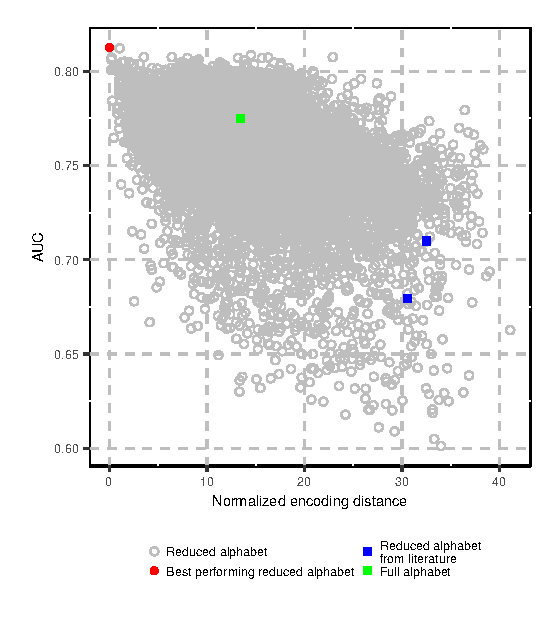
\includegraphics{figures/ed_AUC.eps}}
\caption{The encoding distance and AUC of reduced alphabets studied in the 
cross-validation. 
%Red circle: classifier employing best encoding of amino acid. Green square: 
%classifier using full amino acid alphabet. Blue square: classifiers employing 
%encodings from literature. 
Classifiers with the smallest encoding distance to the best classifier have 
the highest AUC.}\label{fig:ed_AUC}
\end{figure}

% latex table generated in R 3.2.3 by xtable 1.8-2 package
% Tue Mar  8 14:20:53 2016
\begin{table}[ht]
\centering
\caption{The best-performing encoding.} 
\label{tab:best_enc}
\begin{tabular}{cl}
\toprule
Subgroup ID & Amino acids \\ 
\midrule
  1 & G \\ 
\rowcolor[gray]{0.85}  2 & K, P, R \\ 
3 & I, L, V \\ 
\rowcolor[gray]{0.85}  4 & F, W, Y \\ 
5 & A, C, H, M \\ 
\rowcolor[gray]{0.85}  6 & D, E, N, Q, S, T \\ 
\bottomrule
\end{tabular}
\end{table}


\begin{figure}[!tpb]
\centerline{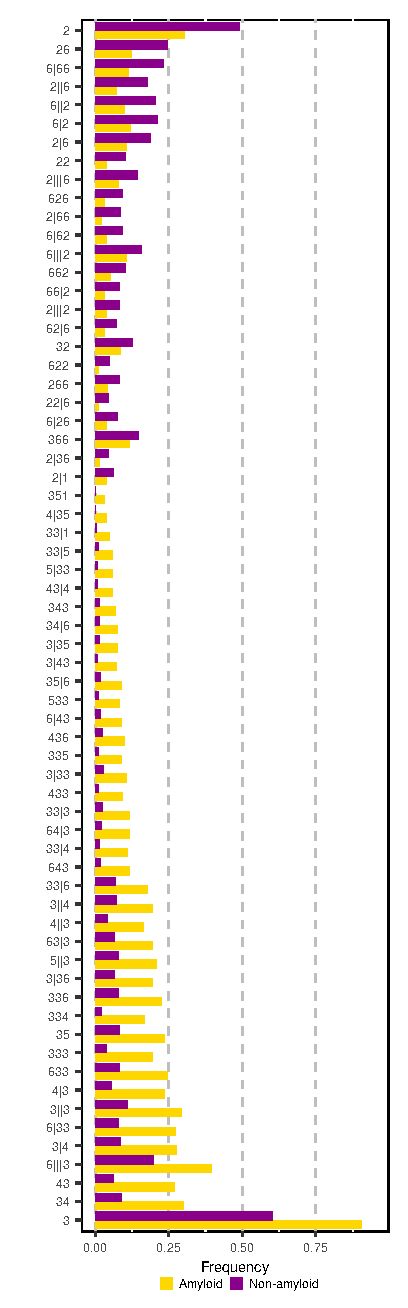
\includegraphics{figures/ngrams.eps}}
\caption{The frequency of important n-grams used by the best-performing classifier 
in amyloid and non-amyloid sequences. The elements of n-grams 
are amino acids encoded using the best-performing reduced amino acid 
alphabet (see Tab.~\ref{tab:best_enc}). A vertical bar 
represents a gap in a n-gram.}\label{fig:ngrams}
\end{figure}

The reduced amino acid alphabet chosen during the analysis has six subgroups 
(Tab.~\ref{tab:best_enc}). Two subgroups, 3 and 4 contain strongly hydrophobic 
amino acids, while 1 and 5 are mostly hydrophilic. In addition to this, subgroup 
1 and 4 have amino acid with the highest average flexibility. The least flexible 
amino acids are in subgroup 5. The most polarizable amino acids belong to 
subgroup 4, while the lowest polarizability is typical for glycine, the only 
amino acid in subgroup 1. The glycine has also the highest thermodynamic beta 
sheet propensity, which has the lowest values for subgroups 3 and 4.

  In total, eleven combinations of physicochemical properties created the best 
performing reduced amino acid alphabet. Only four features appeared in all 
combinations: hydrophobicity index~\citep{argos_structural_1982}, average 
flexibility indices~\citep{bhaskaran_positional_1988}, polarizability 
parameter~\citep{charton_structural_1982} and thermodynamic $\beta$-sheet 
propensity~\citep{kim_thermodynamic_1993}.

  We calculated encoding distances between the best-performing reduced amino 
acid alphabet and other encodings (Fig.~\ref{fig:ed_AUC}). To compute the scale 
factor, we used described above features common for all encodings identical to 
the best-performing one. The value of AUC is significantly lower for more 
% * <kotulska@gmail.com> 2016-03-29T15:01:01.743Z:
%
% > encodings identical to 
% > the best-performing one.
%
% co to są kodowania identyczne z najlepszym? Jest ich więcej najlepszych?
%
% ^ <michalburdukiewicz@gmail.com> 2016-03-31T17:13:57.599Z:
%
% różne cechy fizykochemiczne mogą dać takie samo kodowanie aminokwasów, co znaczy, że część alfabetów miała swoje duplikaty. Alfabet, który miał najlepszy performance mógł powstać z 11 różnych kombinacji cech fizykochemicznych. Akapit wyżej omawiamy cechy fizykochemiczne wspólne, które wystąpiły w każdej z tych kombinacji.
%
% ^.
distant encodings ($-0.4370$ Pearson's correlation coefficient, p-value smaller 
than $2.2 \times 10^{-16}$). Such relationship between AUC and encoding distance 
confirms that only reduced alphabets sufficiently similar to the best-performing 
encoding are able to remove unnecessary diversity while preserving information 
important for recognition of amyloids.

 We selected 65 n-grams that have p-values smaller than 0.05 in the all folds in 
all repetitions of cross-validation regardless of the length of sequences in the 
training set (see Fig.~\ref{fig:ngrams}). The frequency of the n-grams was 
computed for all sequences derived from AmyLoad database. The n-grams typical 
for amyloidogenic sequences (with the highest frequency in amyloids) incorporate 
mostly highly hydrophobic, typical for $\beta$-structures amino acids from 
subgroups 3 and 4. The important n-grams occurring frequent in amyloids often 
have repeats of 3, suggesting that the presence of amino acids belonging to this 
subgroup might be one of the most effective predictors of amyloidogenicity.

  N-grams typical for non-amyloidogenic peptides have mostly elements 
belonging to subgroups 2 and 6. The amino acids of these subgroups are strongly 
hydrophilic and highly flexible, in the opposite to the residues typical for 
amyloids.

\subsection{Benchmark of AmyloGram}

% latex table generated in R 3.2.3 by xtable 1.8-2 package
% Tue Mar  8 14:17:55 2016
\begin{table}[ht]
\centering
\caption{Results of benchmark on \textit{pep424} data set for AmyloGram, 
PASTA2, FoldAmyloid and random forest predictor learned on n-grams extracted 
without any amino acid encoding from the sequences of the length specified in 
the brackets.} 
\label{tab:bench_summary}
\begin{tabular}{ccccc}
  \toprule
Classifier & AUC & MCC & Sensitivity & Specificity \\ 
  \midrule
AmyloGram & \textbf{0.8972} & \textbf{0.6307} & \textbf{0.8658} & 0.7889 \\ 
   \rowcolor[gray]{0.85}PASTA2 & 0.8550 & 0.5227 & 0.7987 & 0.7444 \\ 
  FoldAmyloid & 0.7351 & 0.4526 & 0.7517 & 0.7185 \\ 
   \rowcolor[gray]{0.85}full alphabet (6) & 0.8411 & 0.5427 & 0.4966 & 
\textbf{0.9593} \\ 
  full alphabet (6-10) & 0.8581 & 0.5698 & 0.7517 & 0.8259 \\ 
   \rowcolor[gray]{0.85}full alphabet (6-15) & 0.8610 & 0.5490 & 0.8188 & 
0.7519 
\\ 
   \bottomrule
\end{tabular}
\end{table}

The benchmark covered Amylogram as well as two best-performing peer-reviewed 
predictors of amyloidogenicity (PASTA2~\citep{walsh_pasta_2014} and 
FoldAmyloid~\citep{garbuzynskiy_foldamyloid:_2010}). We analyzed Area Under the 
Curve (AUC), Matthew's Correlation Coefficient (MCC), Sensitivity and 
Specificity (see Tab.~\ref{tab:bench_summary}).
    
  Interestingly, the n-gram extraction method was efficient enough to produce 
classifiers able to outperformed published methods. Two of three n-gram based 
classifiers trained on the full alphabet have AUC higher than PASTA2 and all 
three were more successful than FoldAmyloid. They also maintained they high 
Specificity as seen previously during cross-validation.
    
  Although the proposed n-gram extraction creates efficient classifiers, the 
encoding of amino acids further increases the prediction of amyloidogenicity. 
AmyloGram has the highest AUC, MCC and Sensitivity among all tested classifiers. 
Is has lower specificity than two classifiers trained on the full alphabet, but 
still outperforms other published method in this category. It is important to 
highlight that AmyloGram is the most  of analyzed classifiers, having 
the best Specificity/Sensitivity trade-off, as indicated by the value of MCC.



\section{Conclusion}

Thanks to the reduction of amino acid alphabet, we were able to create the 
efficient predictor of amyloidogenic sequences called AmyLoad. One of the 
strength of our approach is its highly interpretable outcome, which hopefully 
sheds new light on the process of amyloid aggregation.

  The idea of using the reduced amino acid alphabets is not new, but we employed 
innovative framework to generate and validate several thousands of possible 
amino acid encodings. Due to this approach, we are able to specify important 
physicochemical properties that define the best-performing alphabet.  We 
confirmed the relevance of properties commonly associated with amyloidogenicity 
as hydrophobicity and discover new ones, as flexibility.  

  Our analysis was completed with the extraction of important n-grams, which 
might be interpreted as short motifs highly relevant to amyloidogenicity or 
nonamyloidogenicity of the peptide. 65 important n-grams revealed that mostly 
alifatic and nonpolar amino acids as isoleucine, leucine and valine are 
responsible for the hydrophobic character of amyloids. Only in their 
neighborhood, the presence of aromatic and hydrophobic amino acids 
(phenylalanine, tyrosine, tryptophan) is also a sign of a potential amyloid. 

  Since the best-performing classifier was trained on the alphabet of length 
six, but still outperformed predictors learning on the raw amino acid sequence, 
we cannot surely determine the optimal length of a reduced amino acid alphabet 
for detection of amyloids. It is plausible that such alphabet is longer than 
six residues. Nevertheless, the alphabet of length six is enough to find 
n-grams separating efficiently amyloids and non-amyloids. 

% * <kotulska@gmail.com> 2016-03-29T14:58:53.648Z:
%
% Trzeba streścić najważniejsze kroki analizy i podsumować wyniki
%
% ^.

\section*{Acknowledgments}

\noindent Calculations were carried out in Wroclaw Center for Networking 
and Supercomputing (http://www.wcss.pl), grant No. 347 and by KNOW Consortium.

\section*{Funding}

This research was partially funded by the KNOW Consortium.

\bibliographystyle{natbib}
%\bibliographystyle{achemnat}
%\bibliographystyle{plainnat}
%\bibliographystyle{abbrv}
%\bibliographystyle{bioinformatics}
%
%\bibliographystyle{plain}
%
\bibliography{amyloids}
\end{document}
